
% This work is licensed under the Creative Commons Attribution-Share Alike 2.0 France License.
% To view a copy of this license, visit http://creativecommons.org/licenses/by-sa/2.0/fr/legalcode
% or send a letter to Creative Commons, 171 Second Street, Suite 300, San Francisco, California, 94105, USA.

\chapter{Réponses aux «~À vous de jouer~»\label{annexe:reponses}}


Vous trouverez ici les réponses aux questions posées dans la plupart des chapitres dans la section «~À vous de jouer~». 

\section{Réponses aux cas pratiques de la \autoref{pratique:8}\label{reponses:8}}
\begin{enumerate}
\item La réponse à l'\textbf{exercice 1} devrait ressembler à ce qui suit:\\

\begin{small}
\begin{Verbatim}[frame=single,rulecolor=\color{mbleu}, label=à taper]
>>> jouets= [ 'Lego', 'Playmo', 'mandala', 'vélo' ]
>>> plats = [ 'crêpes', 'gaufres', 'betterave' ]
>>> préférés = jouets + plats
>>> print(préférés)
['Lego', 'Playmo', 'mandala', 'vélo', 'crêpes', 'gaufres', 'betterave']
\end{Verbatim}
%\rm
\end{small}
\item  La réponse à l'\textbf{exercice 2} est simplement d'ajouter le résultat de «~\texttt{3*25}~» et le résultat de «~\texttt{10*32}~». L'équation suivant montre le résultat de cette équation:

\begin{Verbatim}[frame=single,rulecolor=\color{mbleu}, label=à taper]
>>> print(3 * 25 + 10 * 32)
395
\end{Verbatim}
\rm
\emph{Ce qui fait beaucoup de friandises!}\\

Néanmoins, si vous avez suivi la partie sur l'usage de parenthèses dans le chapitre \ref{chap:8}, vous pouvez avoir décidé de mettre des parenthèses dans cette équation. Vous devriez avoir fait quelque chose comme:
\tt
\begin{Verbatim}[frame=single,rulecolor=\color{mbleu}, label=à taper]
>>> print((3 * 25) + (10 * 32))
395
\end{Verbatim}
\rm

La réponse est la même, car la multiplication est faite avant l'addition. Dans les deux équations les deux multiplications sont faites en premier et les résultats sont additionnés. Malgré tout la seconde équation est peut-être légèrement meilleure que la première. En effet, l'ordre des opérations est immédiatement évident pour le lecteur. Un programmeur moins compétent (qui ne connaîtrait pas aussi bien l'ordre des opérations) pourrait penser que dans la première équation vous multipliez 3 par 25, puis additionnez 10 et multipliez le résultat par 32 (la réponse complément fausse est 2720). Avec les parenthèses il est un peu plus simple de comprendre ce qui est calculé en premier.

\item  La réponse à l'\textbf{exercice 2} devrait ressembler à:
\tt
\begin{Verbatim}[frame=single,rulecolor=\color{mbleu}, label=à taper]
>>> prénom = 'Morgane'
>>> nom = 'Paul'
>>> print('Mon nom est %s %s.' % (prénom, nom))
Mon nom est Morgane Paul.
\end{Verbatim}
\rm

\end{enumerate}

\section{Réponses aux cas pratiques de la \autoref{pratique:tortues}\label{reponses:tortues}}
\begin{enumerate}
\item La réponse à l'\textbf{exercice 1} devrait ressembler à ce qui suit: un rectangle est semblable à un carré mis à part que deux côtés peuvent être plus longs que les deux autres. En disant à la tortue de faire les actions suivantes, vous pouvez aisément dessiner un rectangle:
\begin{itemize}
 \item avancer d'un certain nombre de points;
 \item tourner à angle droit;
 \item avancer d'un certain nombre de points;
 \item tourner à angle droit dans le même sens que la première rotation;
 \item avancer du même nombre de points que pour le premier déplacement;
 \item tourner à angle droit dans le même sens que la première rotation;
 \item avancer du même nombre de points que pour le deuxième déplacement.
\end{itemize}

Par exemple, le code suivant tracera un rectangle que vous pouvez voir sur la \autoref{fig46}.
\begin{Verbatim}[frame=single,rulecolor=\color{mbleu}, label=à taper]
import turtle

tortue = turtle.Pen()
tortue.forward(150)
tortue.left(90)
tortue.forward(50)
tortue.left(90)
tortue.forward(150)
tortue.left(90)
tortue.forward(50)
\end{Verbatim}


\begin{figure}[h!t]
\begin{center}
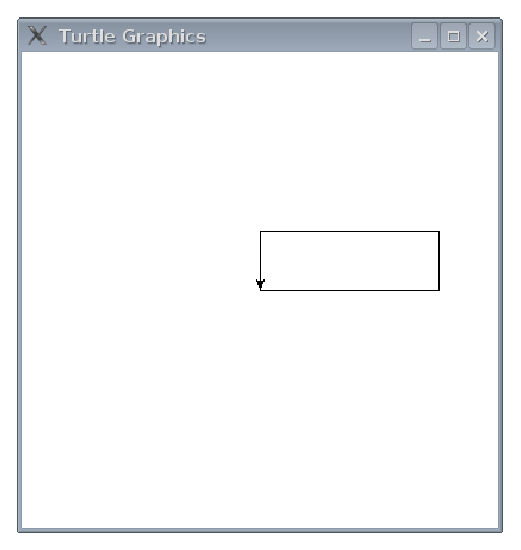
\includegraphics[width=82mm]{images/rectangletortue.eps}
\end{center}
\caption{Tortue dessinant un rectangle.}\label{fig46}
\end{figure}

\item La réponse à l'\textbf{exercice 2} devrait ressembler à ce qui suit:

Un triangle est un peu plus compliqué à dessiner car vous avez besoin de connaître plus d'informations sur les angles et les longueurs des côtés. Si vous n'avez pas étudié les angles à l'école cela pourrait être un peu plus difficile que vous ne vous y attendiez. Vous pouvez dessiner un triangle simple (voir la \autoref{fig:trianglesimple} avec le code suivant:

\begin{Verbatim}[frame=single,rulecolor=\color{mbleu}, label=à taper]
import turtle

tortue = turtle.Pen()
tortue.forward(100)
tortue.left(135)
tortue.forward(70)
tortue.left(90)
tortue.forward(70)
\end{Verbatim}

\begin{figure}[h!t]
\begin{center}
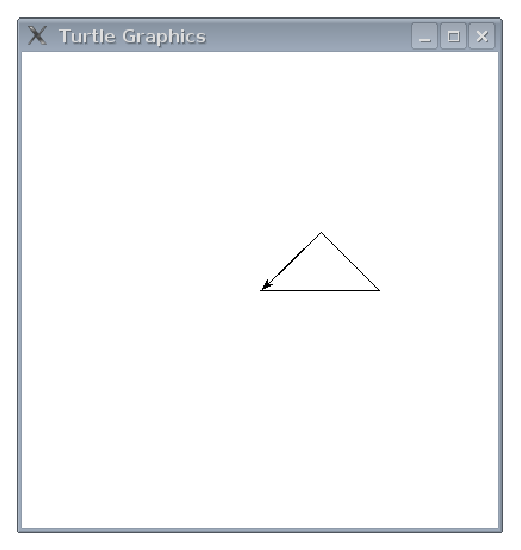
\includegraphics[width=82mm]{images/trianglesimple.eps}
\end{center}
\caption{La tortue dessine un triangle}\label{fig:trianglesimple}
\end{figure}

\end{enumerate}

\section{Réponses aux cas pratiques de la \autoref{pratique:boucles}\label{reponses:boucles}}
\begin{enumerate}
\item La réponse à l'\textbf{exercice 1} est que seule la chaîne \texttt{x vaut 0} sera affichée. Regardons le code en détail pour comprendre pourquoi.
\begin{Verbatim}[frame=single,rulecolor=\color{gray}, label=ne pas taper]
>>> for x in range(0, 20):
... 	print('x vaut %s' % x)
... 	if x < 9:
... 		break
x vaut 0
\end{Verbatim}

La raison en est que durant la première itération la valeur de variable \texttt{x} est zéro. Comme zéro vaut moins que neuf, la commande \texttt{break} est lancée et fait sortir de la boucle.

\item Pour répondre à l'\textbf{exercice 2} je vous propose d'écrire un petit programme qui va calculer le nombre de nénuphars chaque jour et l'afficher. Quand le nombre de nénuphars dépassera mille il suffit d'arrêter la boucle.

Pour information voila à quoi peut ressembler un tel programme.
\begin{Verbatim}[frame=single,rulecolor=\color{gray}, label=ne pas taper]
>>> jours = 0
>>> nénuphars = 1
>>> while nénuphars < 1000:
...     jours+=1
...     nénuphars*=2 
...     print('Au bout de %s jours, il y a %s nénuphars.' % (jours, nénuphars))
... 
Au bout de 1 jours, il y a 2 nénuphars.
Au bout de 2 jours, il y a 4 nénuphars.
Au bout de 3 jours, il y a 8 nénuphars.
Au bout de 4 jours, il y a 16 nénuphars.
Au bout de 5 jours, il y a 32 nénuphars.
Au bout de 6 jours, il y a 64 nénuphars.
Au bout de 7 jours, il y a 128 nénuphars.
Au bout de 8 jours, il y a 256 nénuphars.
Au bout de 9 jours, il y a 512 nénuphars.
Au bout de 10 jours, il y a 1024 nénuphars.
>>> print("Il faut seulement %s jours pour que le lac soit envahi" % jours)
Il faut seulement 10 jours pour que le lac soit envahi
\end{Verbatim}

Aux deux premières lignes nous initialisons les variables «~\verb+nénuphars+~» à un et «~\verb+jours+~» à zéro.  
À la troisième ligne nous créons une boucle «~tant que~» en utilisant comme condition d'arrêt que le nombre de nénuphars devient supérieur ou égal à mille. Puis, dans le bloc nous augmentons le nombre de jours de un jour à chaque pas et multiplions le nombre de nénuphars par deux à chaque pas. Enfin, nous affichons le résultat du calcul de chaque pas. Une fois sortis de la boucle nous synthétisons le résultat. 
\end{enumerate}

\section{Réponses aux cas pratiques de la \autoref{pratique:recyclage}\label{reponses:recyclage}}
\begin{enumerate}
\item La réponse à l'\textbf{exercice 1} devrait ressembler à ce qui suit: 

\end{enumerate}

\subsection*{Chapter \ref{ch:sortoflikerecycling}}

\noindent
1. Turning the for-loop into a function is actually quite easy.  The function will look something like this:

\begin{listing}
\begin{verbatim}
>>> def calculate_interest(amount, rate):
...     for year in range(1, 11):
...         interest = amount * rate
...         print('interest earned for savings %s for year %s is %s' % 
...             (amount, year, interest))
...         amount = amount + interest
\end{verbatim}
\end{listing}

If you compare the function with the code above, you might notice that, apart from the first line, there's only one change to the original code (0.03 is now the parameter \texttt{rate}). Because \texttt{amount} was already a variable, there's no change required when it becomes a parameter. You'll find the output is also the same when you run the function:

\begin{listing}
\begin{verbatim}
>>> calculate_interest(100, 0.03)
interest earned for savings 100 for year 1 is 3.0
interest earned for savings 103.0 for year 2 is 3.09
interest earned for savings 106.09 for year 3 is 3.1827
interest earned for savings 109.2727 for year 4 is 3.278181
interest earned for savings 112.550881 for year 5 is 3.37652643
interest earned for savings 115.92740743 for year 6 is 3.4778222229
interest earned for savings 119.405229653 for year 7 is 3.58215688959
interest earned for savings 122.987386542 for year 8 is 3.68962159627
interest earned for savings 126.677008139 for year 9 is 3.80031024416
interest earned for savings 130.477318383 for year 10 is 3.91431955149
\end{verbatim}
\end{listing}

\noindent
2. Changing the function to pass in the year as a parameter also involves only minor changes:

\begin{listing}
\begin{verbatim}
>>> def calculate_interest(amount, rate, years):
...     for year in range(1, years):
...         interest = amount * rate
...         print('interest earned for savings %s for year %s is %s' %
...             (amount, year, interest))
...         amount = amount + interest
\end{verbatim}
\end{listing}

\noindent
We can now easily change the starting amount, the rate of interest and the number of years:

\begin{listing}
\begin{verbatim}
>>> calculate_interest(1000, 0.05, 6)
interest earned for savings 1000 for year 1 is 50.0
interest earned for savings 1050.0 for year 2 is 52.5
interest earned for savings 1102.5 for year 3 is 55.125
interest earned for savings 1157.625 for year 4 is 57.88125
interest earned for savings 1215.50625 for year 5 is 60.7753125
\end{verbatim}
\end{listing}

\noindent
3. The mini-program is a bit more complicated than the functions we've already created.  First we need to import the sys module so we can ask for input.  Then we need to prompt the user of our program for each of the values.  Apart from that, the function stays roughly the same:

\begin{listing}
\begin{verbatim}
>>> import sys
>>> def calculate_interest():
...     print('Enter the amount you have to save')
...     amount = float(sys.stdin.readline())
...     print('Enter the interest rate')
...     rate = float(sys.stdin.readline())
...     print('Enter the number of years')
...     years = int(sys.stdin.readline())
...     for year in range(1, years):
...         interest = amount * rate
...         print('interest earned for savings %s for year %s is %s' % 
...             (amount, year, interest))
...         amount = amount + interest
\end{verbatim}
\end{listing}

\noindent
When we run the function, we'll see something like the following:

\begin{listingignore}
\begin{verbatim}
>>> calculate_interest()
Enter the amount you have to save
500
Enter the interest rate
0.06
Enter the number of years
12
interest earned for savings 500.0 for year 1 is 30.0
interest earned for savings 530.0 for year 2 is 31.8
interest earned for savings 561.8 for year 3 is 33.708
interest earned for savings 595.508 for year 4 is 35.73048
interest earned for savings 631.23848 for year 5 is 37.8743088
interest earned for savings 669.1127888 for year 6 is 40.146767328
interest earned for savings 709.259556128 for year 7 is 42.5555733677
interest earned for savings 751.815129496 for year 8 is 45.1089077697
interest earned for savings 796.924037265 for year 9 is 47.8154422359
interest earned for savings 844.739479501 for year 10 is 50.6843687701
interest earned for savings 895.423848271 for year 11 is 53.7254308963
\end{verbatim}
\end{listingignore}

\subsection*{Chapter \ref{ch:turtlesgalore}}

\noindent
1. There's a hard way to draw an octagon, and an easy way.  The hard way, isn't hard because it's complicated.  It's hard because it requires more typing:

\begin{listing}
\begin{verbatim}
import turtle
t = turtle.Pen()
>>> t.forward(50)
>>> t.right(45)
>>> t.forward(50)
>>> t.right(45)
>>> t.forward(50)
>>> t.right(45)
>>> t.forward(50)
>>> t.right(45)
>>> t.forward(50)
>>> t.right(45)
>>> t.forward(50)
>>> t.right(45)
>>> t.forward(50)
>>> t.right(45)
>>> t.forward(50)
\end{verbatim}
\end{listing}

\noindent
You can see from that code that we tell the turtle to move forward 50 pixels, then turn right 45 degrees.  We do this 8 times.  Which is a lot of time.  The easier way to draw an octagon is the following code (which produces the octagon in figure~\ref{fig48}):

\begin{listing}
\begin{verbatim}
>>> for x in range(0,8):
...     t.forward(50)
...     t.right(45)
\end{verbatim}
\end{listing}

\begin{figure}
\begin{center}
%\includegraphics[width=82mm]{figure48.eps}
\end{center}
\caption{Turtle drawing an octagon.}\label{fig48}
\end{figure}

\noindent
2.  If you take another look at the other functions in Chapter~\ref{ch:turtlesgalore}, you'll already see how to create a filled shape. We can convert the octagon code into a function that takes a colour, but we'll also want to reuse the hexcolour function 

\begin{listing}
\begin{verbatim}
>>> def octagon(red, green, blue):
...     t.color(red, green, blue)
...     t.begin_fill()
...     for x in range(0,8):
...         t.forward(50)
...         t.right(45)
...     t.end_fill()
\end{verbatim}
\end{listing}

We set the colour, then turn filling on.  Then we run the for loop to draw the octagon, finally we switch filling back off again to fill in the shape. How about a blue octagon (see figure~\ref{fig49}):

\begin{listing}
\begin{verbatim}
>>> octagon(0, 0, 1)
\end{verbatim}
\end{listing}

\begin{figure}
\begin{center}
%\includegraphics[width=82mm]{figure49.eps}
\end{center}
\caption{Turtle drawing a blue octagon.}\label{fig49}
\end{figure}
\newpage
